%%%% Better Poster latex template example v1.0 (2019/04/04)
%%%% GNU General Public License v3.0
%%%% Rafael Bailo
%%%% https://github.com/rafaelbailo/betterposter-latex-template
%%%% 
%%%% Original design from Mike Morrison
%%%% https://twitter.com/mikemorrison

\documentclass[a0paper,fleqn]{betterposter}

%%%% Uncomment the following commands to customise the format

%% Setting the width of columns
% Left column
\setlength{\leftbarwidth}{0.2\paperwidth}
% Right column
\setlength{\rightbarwidth}{0.2\paperwidth}

%% Setting the column margins
% Horizontal margin
\setlength{\columnmarginvertical}{0.007\paperheight}
% Vertical margin
\setlength{\columnmarginhorizontal}{0.03\paperheight}
% Horizontal margin for the main column
\setlength{\maincolumnmarginvertical}{0.03\paperheight}
% Vertical margin for the main column
\setlength{\maincolumnmarginhorizontal}{0.05\paperheight}

%% Changing font sizes
% Text font
%\renewcommand{\fontsizestandard}{\fontsize{28}{35} \selectfont}
% Main column font
\renewcommand{\fontsizemain}{\fontsize{40}{50} \selectfont}
% Title font
\renewcommand{\fontsizetitle}{\fontsize{60}{70} \selectfont}
% Author font
\renewcommand{\fontsizeauthor}{\fontsize{35}{45} \selectfont}
% Section font
%\renewcommand{\fontsizesection}{\fontsize{28}{35} \selectfont}

%% Changing font sizes for a specific text segment
% Place the text inside brackets:
% {\fontsize{28}{35} \selectfont Your text goes here}

%% Changing colors
% Background of side columns
%\renewcommand{\columnbackgroundcolor}{black}
% Font of side columns
%\renewcommand{\columnfontcolor}{gray}
% Background of main column
%\renewcommand{\maincolumnbackgroundcolor}{empirical}
%\renewcommand{\maincolumnbackgroundcolor}{theory}
%\renewcommand{\maincolumnbackgroundcolor}{methods}
\usepackage{xcolor}
\definecolor{lightblue}{RGB}{135, 206, 235}
\renewcommand{\maincolumnbackgroundcolor}{lightblue!75!black}
% Font of main column
%\renewcommand{\maincolumnfontcolor}{gray}
\DeclareFontFamily{U}{skulls}{}
\DeclareFontShape{U}{skulls}{m}{n}{ <-> skull }{}
\newcommand{\skull}{\text{\usefont{U}{skulls}{m}{n}\symbol{'101}}}

\begin{document}	
\betterposter{
\maincolumn{
\title{Gravity’s Influence on Astronauts’ Eyelid and Eyebrow Heights}
\title{\fontsize{55}{65}\selectfont Findings}
\begin{itemize}
    \item \textbf{Individual Variability:} Astronauts' facial features respond differently to microgravity, with varying degrees of change observed.
    \item \textbf{Environmental Influence:} Gravity significantly affects the relationship between eyelid and eyebrow positions, with distinct differences between Earth and space.
    \item \textbf{Microgravity-Induced Changes:} Increased variability in facial measurements in space suggests microgravity impacts astronauts' facial anatomy over time.
    \vspace{1cm}
\end{itemize}
These results have implications for astronaut health during long-term space missions.

\vspace{2cm}  

\begin{minipage}[t]{0.45\textwidth}  % Left sub-column
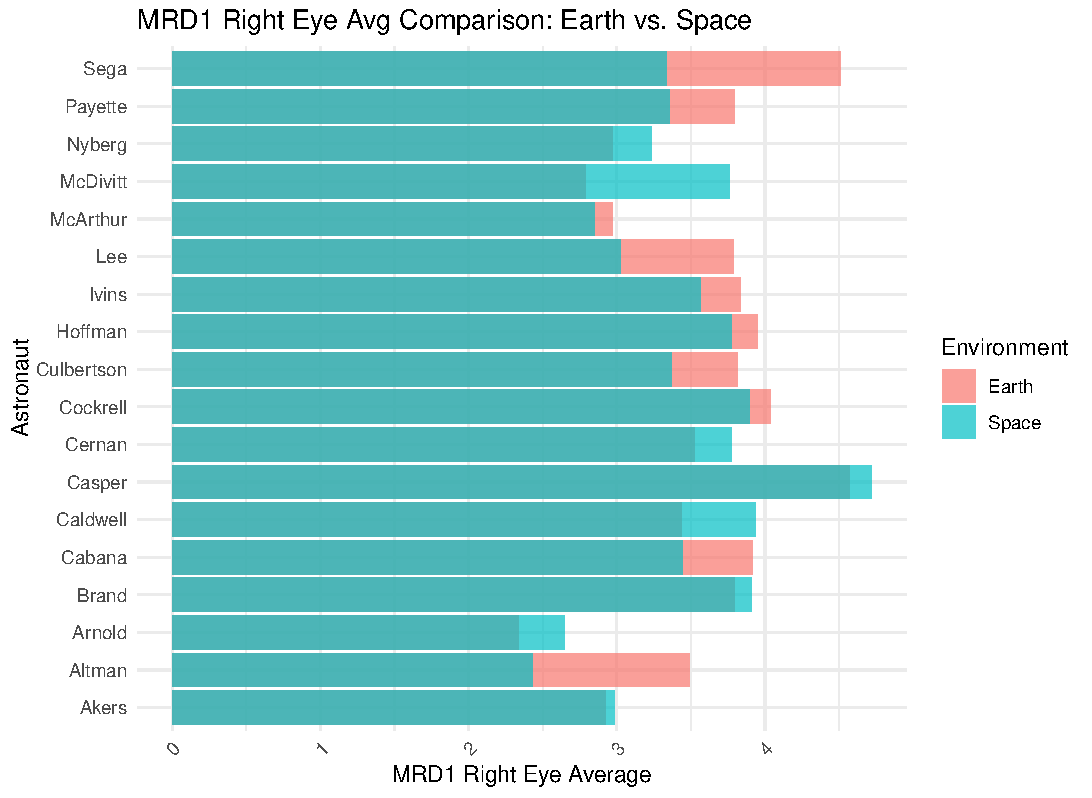
\includegraphics[width=0.9\textwidth]{plots/Bar_Plot.pdf} \\
{\fontsize{30}{40}\selectfont 
\begin{itemize}
    \item \textbf{Demonstrates the complexity of individual responses to microgravity.}
    \item \textbf{Shows that MRD1 measurements vary between Earth and space conditions.}
\end{itemize}
} \\ 

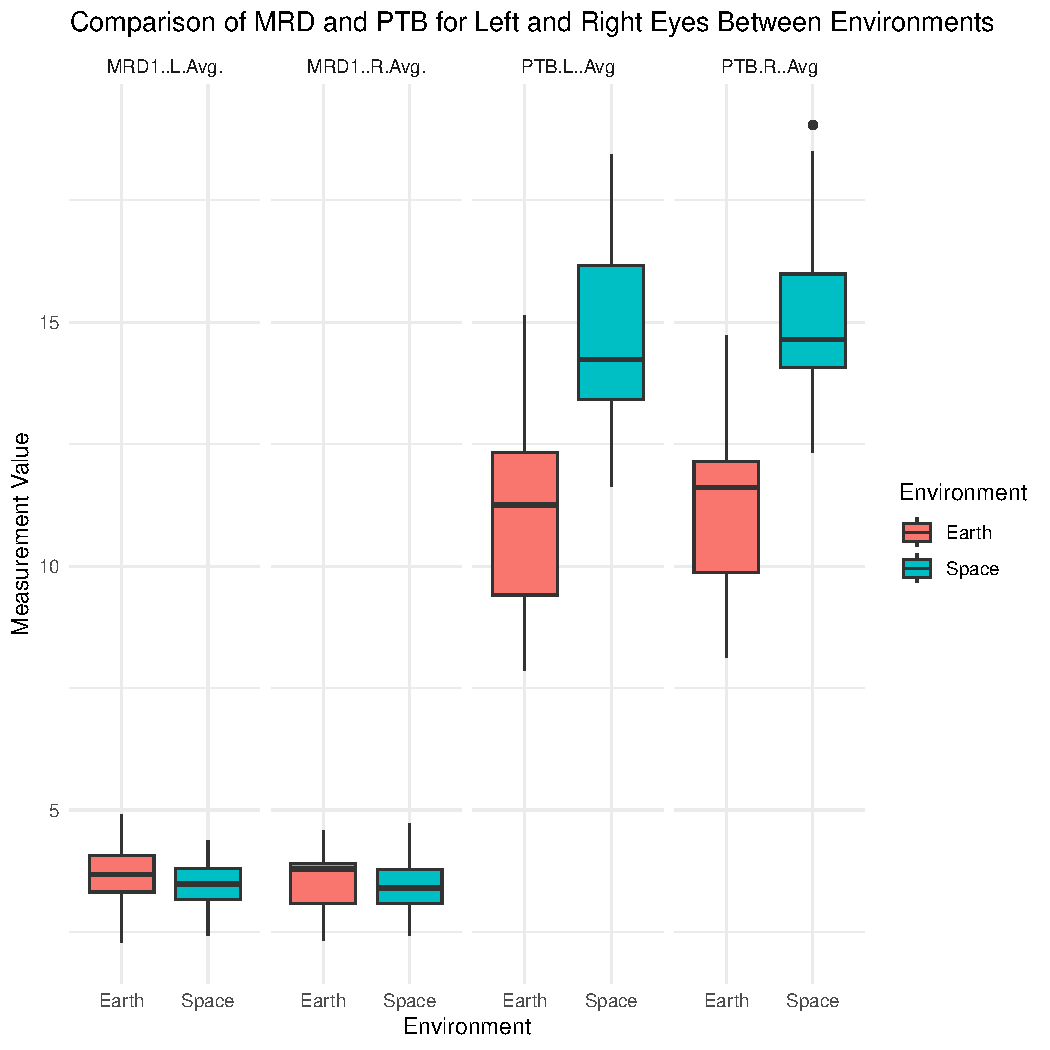
\includegraphics[width=0.9\textwidth]{plots/Boxplot.pdf} \\
{\fontsize{30}{40}\selectfont  
\begin{itemize}
    \item \textbf{Shows variations in measurement spread between Earth and space conditions.}
    \item \textbf{Highlights the potential impact of microgravity on facial measurements.}
\end{itemize}
}
\end{minipage}
\hfill
\begin{minipage}[t]{0.45\textwidth}  % Right sub-column
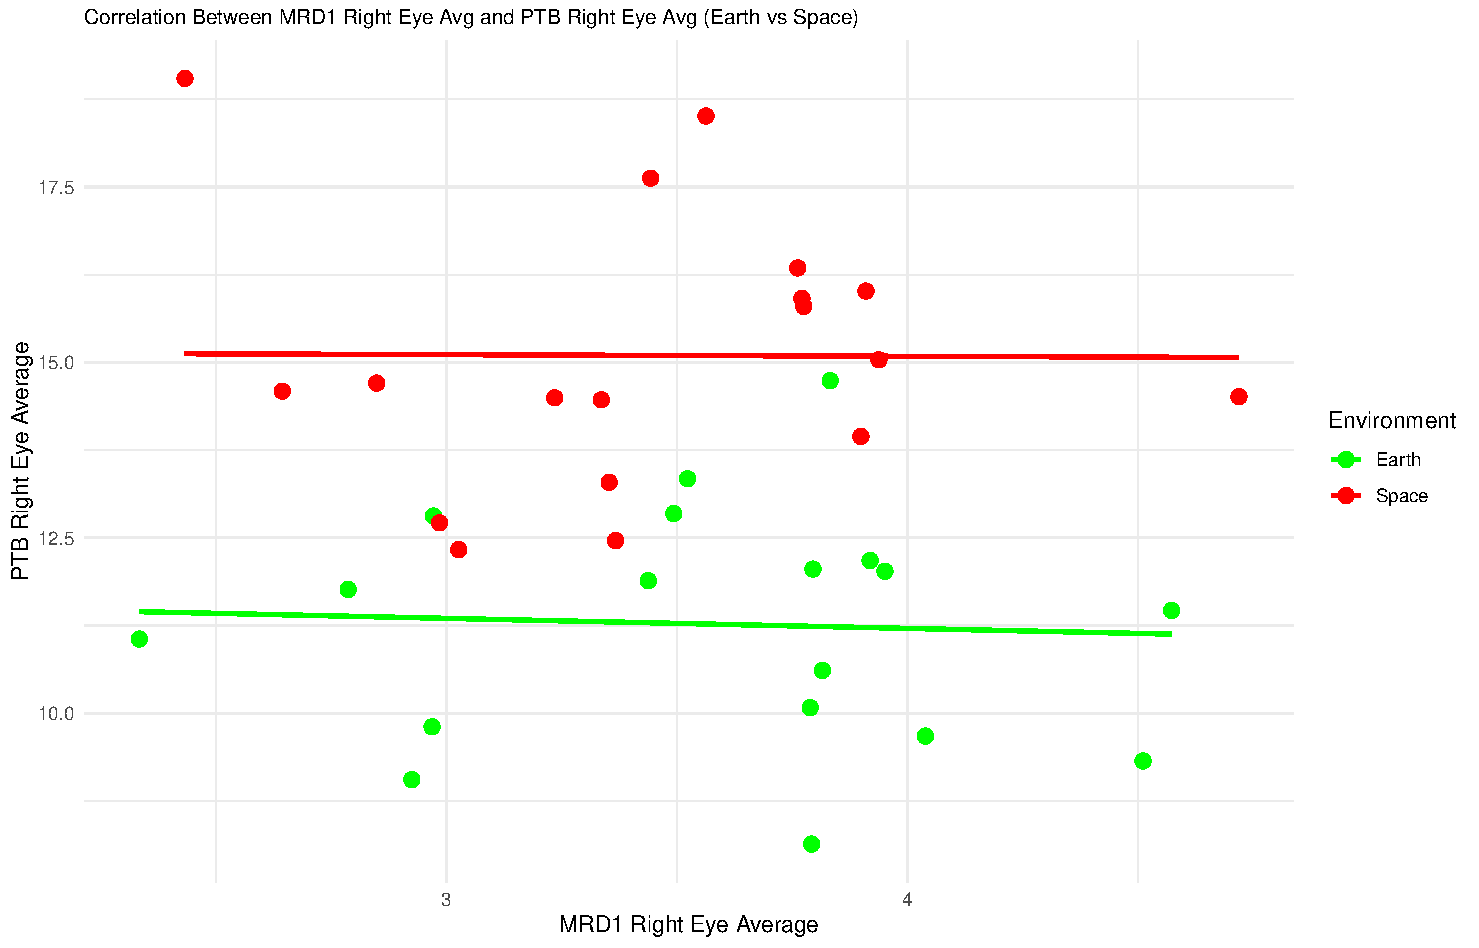
\includegraphics[width=1\textwidth]{plots/Correlation_Plot.pdf} \\ 
{\fontsize{30}{40}\selectfont 
\begin{itemize}
    \item \textbf{Suggests potential correlations between MRD and PTB measurements.}
    \item \textbf{Provides insights into how different eye measurements might change in microgravity.}
\end{itemize}
}  \\ \\
\vspace{2cm}
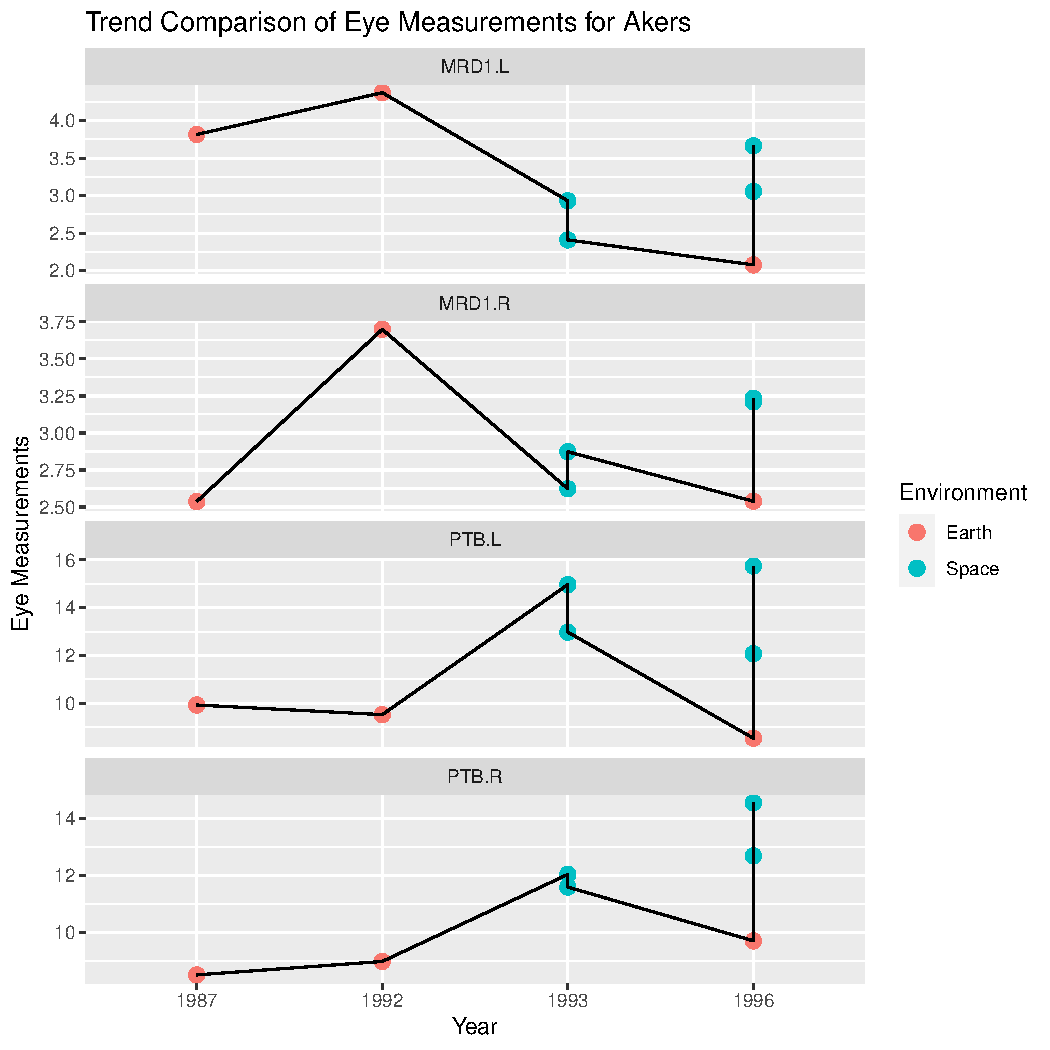
\includegraphics[width=0.8\textwidth]{plots/Line_Plot.pdf} \\
{\fontsize{30}{40}\selectfont 
\begin{itemize}
    \item \textbf{Reveals subtle changes in eye measurements between Earth and space environments.}
    \item \textbf{Demonstrates the potential long-term impacts of microgravity on facial anatomy.}
\end{itemize}
}
\end{minipage}

}{
%%%%%%%% LEFT COLUMN

}{
%%%% Bottom space

%% QR code
%%\qrcode{images/qr-code.png}{images/smartphone}{
%%\textbf{Take a picture} to \\
%%download the full paper
%%}
% Smartphone icon
% Author: Freepik
% Retrieved from: https://www.flaticon.com/free-icon/smartphone_65680

%% Compact QR code (comment the previous command and un-comment this one to switch)
%\compactqrcode{images/qr-code.png}{
%\textbf{Take a picture} to
%\\download the full paper
%}
}
}{
%%%%%%%% LEFT COLUMN

\section{Authors}
\author{Evelyn Yi Tsing Ng}
\author{Jamie Tian}
\author{Qianping Wu}
\author{Katherine Jin}
\author{Xuanang Li}
\author{Yangsheng Xu}


\section{Introduction}
This study investigates how gravity affects facial anatomy, specifically eyelid and eyebrow heights. 

\begin{itemize}
\item \textbf{Eyelid height:} Changes in muscle tension and soft tissue.
\item \textbf{Eyebrow height:} Alterations in muscle tone or vascular structure.
\item \textbf{Correlations:} Shared mechanisms between eyelid and eyebrow adaptations.
\end{itemize}

This research uses a dataset from the Jules Stein Eye Institute, comparing values on Earth and in space. We aim to contribute to the growing body of knowledge about human adaptation to the space by our study.

\section{Methods}
\begin{itemize}
\item \textbf{Data Preparation:} Used a cleaned dataset with splitted names and dates, and no NA value, ensuring consistency in column names.
\item \textbf{Analysis:} Used paired t-tests to compare means and calculated correlations between measurements.
\item \textbf{Visualization:} Box plots, scatter plots, dot plots, and line plots illustrate key differences. \\
\end{itemize}

%% Institution logo
\begin{center}
\includegraphics[width=0.65\textwidth]{images/UCLA_ds_001.png} 
\end{center}

%% This fills the space between the content and the logo
%\vfill

%% Institution logo
%\includegraphics[width=\textwidth]{images/DeptLogo.png}\\

}{
%%%%%%%% RIGHT COLUMN
\section{Applications}
\begin{itemize}
\item \textbf{Astronaut Health Monitoring:} Eyelid and eyebrow metrics as non-invasive health indicators.
\item \textbf{Helmet Design:} Adaptive helmet features to accommodate changes in facial anatomy.
\item \textbf{Medical Applications:} Relevance to aging populations and rehabilitation for bedridden patients.
\end{itemize}

\section{Limitations}
\begin{itemize}
\item \textbf{Small Sample Size:} There is a limit on the generalization of findings to the broader astronaut population.
\item \textbf{Uncontrolled Confounding Variables:} Factors such as age were not explicitly adjusted for in the analysis, which may influence results
\item \textbf{Measurement Variability:} Potential inconsistencies in data collection methods.
\end{itemize} 

\section{Future Directions}
\begin{itemize}
\item \textbf{Larger Sample Sizes:} Expand the study with more astronauts.
\item \textbf{Testing Countermeasures:} Explore facial muscle exercises and artificial gravity.
\item \textbf{Simulated Gravity Studies:}  Conduct parabolic flights and bed rest experiments.
\item \textbf{Machine Learning Analysis:} Develop predictive models for facial changes. \\
\end{itemize} 

\vfill

%% QR code

\textbf{The full study} can be found here:
\begin{center}
\includegraphics[width=0.4\textwidth]{images/qr_code.png}{
}
\end{center}

}
\end{document}
